\documentclass[tikz,border=8pt]{standalone}
\usepackage{amsmath}
\usepackage{pgfplots}
\pgfplotsset{compat=1.18}
\definecolor{ink}{HTML}{21352F}
\definecolor{teal}{HTML}{087F7B}
\definecolor{blue}{HTML}{4B77A8}
\definecolor{gold}{HTML}{C58B2A}
\definecolor{rose}{HTML}{B65A62}
\begin{document}
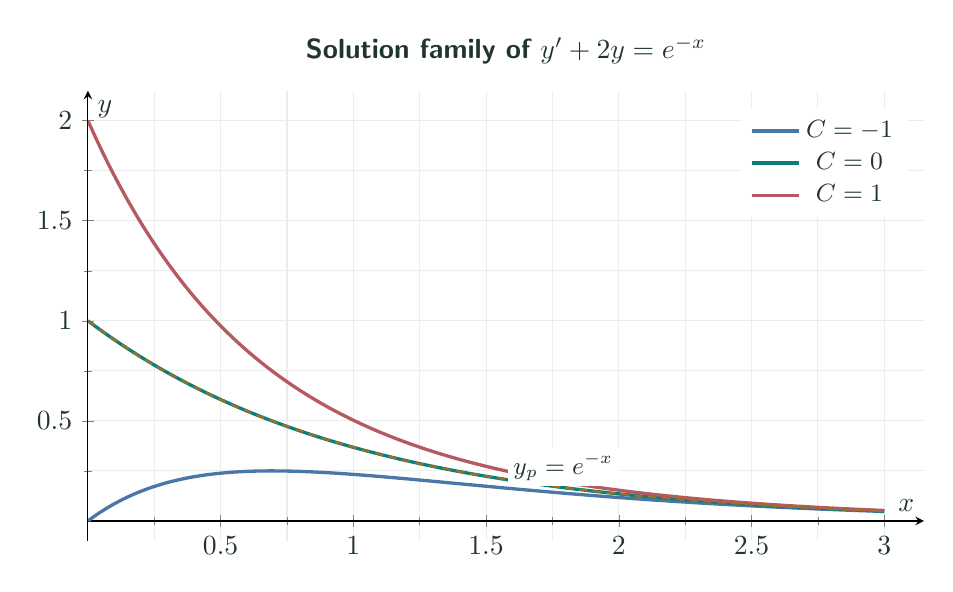
\begin{tikzpicture}[font=\sffamily,text=ink]
  \begin{axis}[
    width=12.2cm,height=7.3cm,
    axis lines=middle,
    xmin=0,xmax=3.15,ymin=-.1,ymax=2.15,
    xlabel={$x$},ylabel={$y$},
    samples=160,domain=0:3,
    grid=both,minor tick num=1,
    grid style={ink!9},
    legend style={draw=none,fill=white,font=\small,at={(.98,.96)},anchor=north east},
    title={\bfseries Solution family of $y'+2y=e^{-x}$}
  ]
    \addplot[blue,very thick] {exp(-x)-exp(-2*x)};
    \addlegendentry{$C=-1$}
    \addplot[teal,very thick] {exp(-x)};
    \addlegendentry{$C=0$}
    \addplot[rose,very thick] {exp(-x)+exp(-2*x)};
    \addlegendentry{$C=1$}
    \addplot[gold!80!black,densely dashed,thick] {exp(-x)};
    \node[anchor=west,fill=white,inner sep=2pt,font=\small]
      at (axis cs:1.58,.27) {$y_p=e^{-x}$};
  \end{axis}
\end{tikzpicture}
\end{document}
